\beginsong{Die Gedanken sind frei}[txt={Hoffmann von Fallersleben nach einem Flugblatt, 1780}, mel={ca. 1810 - 1820}, pfii={115}, pfiii={31}, kssiv={71}]

\beginverse
\endverse

\centering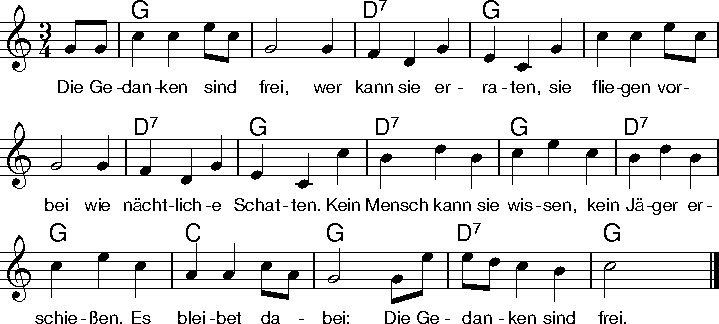
\includegraphics[width=1\textwidth]{Noten/Lied023.pdf}

\beginverse
Ich \[G]denke, was ich will und \[D7]was mich be\[G]glücket, 
und alles in der Still', und \[D7]wie es sich \[G]schicket.
Mein \[D7]Wunsch und Be\[G]gehren kann \[D7]niemand ver\[G]wehren.
Es \[C]bleibet da\[G]bei: Die Ge\[D7]danken sind \[G]frei!
\endverse 

\beginverse
Und ^sperrt man mich ein im ^finsteren ^Kerker,
das alles sind rein ver^gebliche ^Werke,
denn ^meine Ge^danken zer^reißen die ^Schranken
und ^Mauern ent^zwei: Die Ge^danken sind ^frei!
\endverse

\beginverse
Nun ^will ich auf immer den ^Sorgen ent^sagen
und will mich auch nimmer mit ^Grillen mehr ^plagen.
Man ^kann ja im ^Herzen stets ^lachen und ^scherzen
und ^denken da^bei: Die Ge^danken sind ^frei!
\endverse

\beginverse
Ich ^liebe den Wein, mein ^Mädchen vor ^allen,
die tut mir allein am ^Besten ge^fallen.
Ich ^bin nicht al^leine bei ^einem Glas ^Weine;
mein ^Mädchen da^bei: Die Ge^danken sind ^frei!
\endverse

\endsong

\beginscripture{}
Das Lied wurde zuerst in der Sammlung „Lieder der Brienzer Mädchen“ in Bern gedruckt. Im Jahr 1842 wurde das Lied in „Schlesische Volkslieder“ von Hoffmann von Fallersleben und Ernst Richter veröffentlicht. Diese letzte Version stammt von Hoffmann von Fallersleben. Es diente in Zeiten politischer Unterdrückung immer wieder zum Ausdruck der Sehnsucht nach Freiheit und Unabhängigkeit, so zum Beispiel in der Studentenbewegung im 19. Jahrhundert, im Dritten Reich oder während der Berlin-Blockade 1948. 
\endscripture
